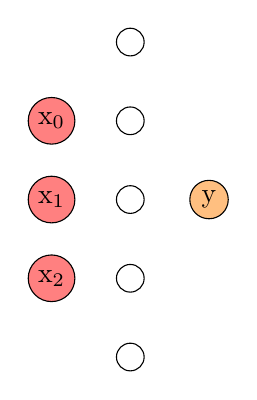
\begin{tikzpicture}[
  inputnode/.style={draw, circle, fill=red!50, inner sep=2pt},
  hiddenunit/.style={draw, circle, minimum size=10pt},
  outnode/.style={draw, circle, fill=orange!50, inner sep=2pt},
]
  \node[inputnode] (x0) at (0, 1) {$\mathrm{x}_0$};
  \node[inputnode] (x1) at (0, 0) {$\mathrm{x}_1$};
  \node[inputnode] (x2) at (0, -1) {$\mathrm{x}_2$};

  \node[hiddenunit] (h2) at (1, 2) {};
  \node[hiddenunit] (h1) at (1, 1) {};
  \node[hiddenunit] (h0) at (1, 0) {};
  \node[hiddenunit] (h3) at (1, -1) {};
  \node[hiddenunit] (h4) at (1, -2) {};

  \node[outnode] (y0) at (2, 0) {$\mathrm{y}$};
\end{tikzpicture}

